% !TEX root = main.tex

\section{支持向量机}
\subsection{支持向量}
超平面由下列方程决定
\[\vw^\T\vx+b=0\]
样本空间中任意点到超平面的距离为
\[r=\frac{|\vw^\T\vx+b|}{\norm{\vw}}\]

若超平面$(\vx,b)$能将样本正确分类,则
\[\begin{cases}
\vw^\T\vx_i+b\geq +1 & y_i=+1\\
\vw^\T\vx_i+b\leq -1 & y_i=-1
\end{cases}\]
距离超平面最近的使上式成立的点称为支持向量(support vector),两个异类支持向量到超平面的距离之和为
\[\gamma=\frac{2}{\norm{\vw}}\]
被称之为间隔(margin)。
\begin{figure}[H]
\centering
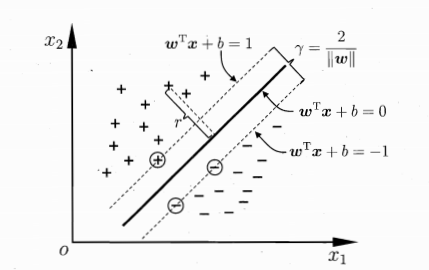
\includegraphics[width=0.6\linewidth]{fig/SVM.png}
\end{figure}

因此为找到最大间隔来划分超平面(分类结果最鲁棒,泛化能力最强),则需要求解下述最优化问题
\begin{maxi*}
{\vw,b}{\frac{2}{\norm{\vw}}}{}{}
\addConstraint{y_i(\vw^\T \vx_i+b)}{\geq 1}{i=1,2,\ldots,m}
\end{maxi*}
显然,为了最大化间隔,只需最大化$\norm{\vw}^{-1}$,等价于最小化$\norm{\vw}^2$,于是上述优化问题可重写为
\begin{maxi*}
{\vw,b}{\frac{1}{2}\norm{\vw}^2}{}{}
\addConstraint{y_i(\vw^\T \vx_i+b)}{\geq 1}{i=1,2,\ldots,m}
\end{maxi*}
此即为支持向量机(Support Vector Machine, SVM)的基本型。

可以用拉格朗日乘子法求对偶问题并得到KKT条件,可利用凸优化的方法进行求解。

支持向量机于[Cortes and Vapnik, 1995]正式发表,由于在文本分类任务中显示出卓越性能[Joachims, 1998],很快成为机器学习主流技术,并直接掀起统计学习(statistical learning)在2000年前后的高潮。

\subsection{核函数}
如果将非线性可分样本从原始空间映射到更高维的特征空间,则可以使其在新的特征空间中线性可分。
\begin{figure}[H]
\centering
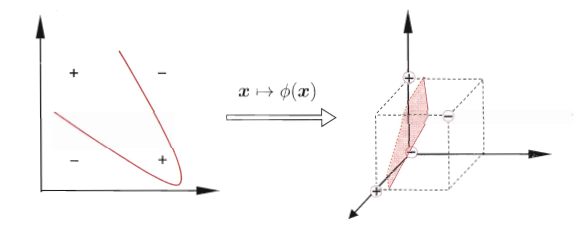
\includegraphics[width=0.6\linewidth]{fig/xor-nonlinear.png}
\end{figure}

由于$\phi(\vx_i)^\T\phi(\vx_j)$的维度可能很高,故设想有这样的核函数(kernel function)
\[\kappa(\vx_i,\vx_j)=\lrang{\phi(\vx_i),\phi(\vx_j)}=\phi(\vx_i)^\T\phi(\vx_j)\]
使得$\vx_i$和$\vx_j$在特征空间的内积等于它们在原始样本空间中通过核函数计算的结果。

几种常见的核函数如下
\begin{center}
\begin{tabular}{ccc}\hline
名称 & 表达式 & 参数\\\hline
线性核 & $\kappa(\vx_i,\vx_j)=\vx_i^\T\vx_j$ & \\
多项式核 & $\kappa(\vx_i,\vx_j)=(\vx_i^\T\vx_j)^d$ & $d\geq 1$为多项式次数\\
高斯核 & $\kappa(\vx_i,\vx_j)=\exp\lrp{-\frac{\norm{\vx_i-\vx_j}^2}{2\sigma^2}}$ & $\sigma>0$为高斯核的带宽(width)\\\hline
\end{tabular}
\end{center}

\subsection{支持向量回归}
支持向量回归(Support vector regression, SVR)允许$f(\vx)$与$y$之间最多有$\eps$的偏差
\begin{figure}[H]
\centering
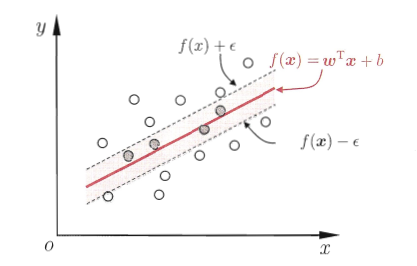
\includegraphics[width=0.6\linewidth]{fig/SVR.png}
\end{figure}

SVR问题可写为
\begin{mini*}
{\vw,b}{\frac{1}{2}\norm{\vw}^2+C\sum_{i=1}^m l_\eps(f(\vx_i)-y_i)}{}{}
\end{mini*}
其中$C$为正则化常数,$l_\eps$为$\eps$-不敏感损失($\eps$-insensitive loss)函数
\[l_\eps(z)=\begin{cases}
0 & |z|\leq \eps\\
|z|-\eps & \text{otherwise}
\end{cases}\]

\subsection{核方法}
基于核函数的学习方法统称为核方法。
最常见是通过``核化''(引入核函数),来将线性学习器扩展为非线性学习器。